\documentclass[a4paper,8pt,twocolumn]{article}
\usepackage{cite}
\usepackage{listings}
\usepackage[T1]{fontenc}
\usepackage{amsmath}
\usepackage{amssymb}
\usepackage{graphicx}
\usepackage[]{circuitikz}
\setlength{\oddsidemargin}{0in}
\setlength{\topmargin}{-.8in}
\setlength{\textheight}{9.7in} \setlength{\textwidth}{6.5in}
\usepackage{color,hyperref}
\definecolor{darkblue}{rgb}{0.0,0.0,0.3}
\hypersetup{colorlinks,breaklinks,
            linkcolor=darkblue,urlcolor=darkblue,
            anchorcolor=darkblue,citecolor=darkblue}
\providecommand*\url[1]{\href{#1}{#1}}
\renewcommand*\url[1]{\href{#1}{\texttt{#1}}}

\newcommand{\bm}[1]{\boldsymbol{#1}}
\newcommand{\bh}[1]{\boldsymbol{\hat{#1}}}
\newcommand{\bt}[1]{\boldsymbol{\tilde{#1}}}
\newcommand{\bbar}[1]{\boldsymbol{\bar{#1}}}
\newcommand{\mbf}[1]{\ensuremath{\mathbf{#1}}}
\newcommand{\ode}[2]{\ensuremath{\frac{\mathrm{d} #1}{\mathrm{d} #2}}}
\newcommand{\odet}[2]{\ensuremath{\tfrac{\mathrm{d} #1}{\mathrm{d} #2}}}
\newcommand{\oden}[3]{\ensuremath{\frac{\mathrm{d}^#3 #1}{\mathrm{d} #2^#3}}}
\newcommand{\pde}[2]{\ensuremath{\frac{\partial #1}{\partial #2}}}
\newcommand{\pdet}[2]{\ensuremath{\tfrac{\partial #1}{\partial #2}}}
\newcommand{\pden}[3]{\ensuremath{\frac{\partial^{#3} #1}{\partial
      #2^{#3}}}}
\newcommand{\sub}[1]{\ensuremath{_{\rm{#1}}}}
\newcommand{\arriba}[1]{\ensuremath{^{\rm{#1}}}}
%
\newcommand{\N}{\ensuremath{\mathbb{N}}}
\newcommand{\R}{\ensuremath{\mathbb{R}}}
\newcommand{\C}{\ensuremath{\mathbb{C}}}
\newcommand{\ee}[1]{\ensuremath{\mathrm{e}^{#1}}}
\newcommand{\hdos}{\ensuremath{\mathrm{H}_2}}
\newcommand{\COdos}{\ensuremath{\mathrm{CO}_2}}
\newcommand{\ATP}{\ensuremath{\mathrm{ATP}}}

\newcommand{\dt}{\ensuremath{\mathrm{d}t}}
\newcommand{\dtau}{\ensuremath{\mathrm{d}\tau}}
\newcommand{\DV}{\ensuremath{\Delta V}}

\DeclareMathOperator{\Li}{\mathcal {L}^{-1}}
\DeclareMathOperator{\Lin}{\mathcal {L}^{-1}}
\DeclareMathOperator{\sinc}{\text{sinc}}
\DeclareMathOperator{\sign}{\mathrm{sign}}
\DeclareMathOperator{\dom}{\mathrm{dom}}
\DeclareMathOperator{\subjectto}{\mathrm{s.t.}}



\newtheorem{remark}{Remark}
\newtheorem{problem}{Problem}
\usepackage[utf8x]{inputenc}
%%

\title{Numerical Experiment\\ Optimization \\ DMKM}
\author{Carlos López Roa\\ \href{mailto:me@mr3m.me}{me@mr3m.me}}
\date{\today}
\pdfinfo{%
  /Title    ()
  /Author   (CLR)
  /Creator  ()
  /Producer ()
  /Subject  ()
  /Keywords ()
}
\begin{document}
\maketitle
%%% Content
\lstset{
language={matlab},
basicstyle=\tiny,
numbers=left,
numberstyle=\tiny,
numbersep=5pt, 
showspaces=false,
showstringspaces=false,
showtabs=False,
frame=false,
%tabsize=.5,
keywordstyle=\bfseries\color{green!40!black},          % keyword style
 commentstyle=\itshape\color{purple!40!black},       % comment style
 identifierstyle=\color{blue},
  stringstyle=\color{orange},
basicstyle=\ttfamily,
captionpos=b}
\lstdefinestyle{matlab}{
language={matlab},
basicstyle=\tiny,
numbers=right,
numberstyle=\tiny,
numbersep=5pt, 
showspaces=false,
showstringspaces=false,
showtabs=False,
frame=single,
tabsize=.5,
keywordstyle=\bfseries\color{green!40!black},          % keyword style
 commentstyle=\itshape\color{purple!40!black},       % comment style
 identifierstyle=\color{blue},
  stringstyle=\color{orange},
basicstyle=\ttfamily,
captionpos=b,
title=\lstname
}
\section*{Abstract}
Given an optimization problem we explore and compare two gradient descent methods, namely: \emph{backtracking line search} and \emph{exact line search}, on which we made a parameter exploration. Manipulation of the optimization problem is done in order to prove some results. 
\section*{Definition}
Consider the problem:
\begin{problem} [Unconstrained minimization ]\label{prob1}
Let $ f : \mathbb{R}^{n} \rightarrow \mathbb{R}$, $\Omega \mapsto T_\Omega$,
\begin{equation}
\begin{aligned}
\min_{x\in \Omega}f(x)&=c^Tx-\sum_{i=1}^m\log(b_i-a_i^Tx),
\end{aligned}
\end{equation}
\end{problem}
%This can be seen as the equivalent problem \cite{Boyd2002}
%\begin{problem}[Unequ]
%
%\end{problem}
Since $T_\Omega\in\mathbb{R}$ we must assure that $f(x)$ takes only real values, thus, we must ensure that $b_i-a_i^Tx>0$, $\forall i, 1\dots m$. This transforms problem \ref{prob1} into the following:
\begin{problem}[Inequality constraint minimization]
Let $ f : \mathbb{R}^{n} \rightarrow \mathbb{R}$, $\Omega \mapsto T_\Omega$,
\begin{equation}
\begin{aligned}
\min_{x\in \Omega}f(x)&=c^Tx-\sum_{i=1}^m\log(b_i-a_i^Tx),\\
\subjectto &\hspace{0.2cm} a_i^Tx - b_i < 0, \hspace{0.2cm} i=1,\dots,m.
\end{aligned}
\end{equation}
\end{problem}
The inequality constraint $a_i^Tx - b_i < 0,$ can be seen as the intersection of $m$ half-planes. If one does not select proper $a,b$, the problem might be unfeasible.  $\Omega$ is then the convex-polytope which is the complement of the intersection of $m$ half-planes. This intersection is open, hence its complement is closed. 

Then, to assure a non-empty domain $\Omega$ we can ask for the following property
\begin{equation}
\begin{aligned}
||A|| \ll ||b||.
\end{aligned}
\end{equation}

That is, the norm of the operator\footnote{The concatanation of all $a_i$} $A=\{a_i\}$, $A\in \mathbb{R}^{m\times n}, A: \mathbb{R}^n \rightarrow \mathbb{R}^m$, must be much much lower than the norm of the vector\footnote{The concatanation of all $b_i$}  $b=\{b_i\}$. 

To find a good initial point $x_0$ we can try to determine the frontier of $\Omega$ ($\partial\Omega$) which is equivalent to finding the left semi-inverse of $A$ in 
\begin{equation}
\begin{aligned}
Ax=b,
\end{aligned}
\end{equation}
which has no trivial solution. Seeing this we must then try to select $x_0$ such that
\begin{equation}
\begin{aligned}
||A||\cdot||x_0|| \ll ||b||.
\end{aligned}
\end{equation}

That is, the product of the norm of the operator $A$ with the norm of the vector $x_0$ must be much much smaller than the norm of the vector $b$.

To implement \emph{gradient descent} method. We must calculate the gradient explicitly which carries

\begin{equation}
\begin{aligned}
\nabla f(x)&=c -\sum_{i=1}^m \frac{a_i}{b_i-a_i^Tx}.
\end{aligned}
\end{equation}

With this said, we have posed the problem to be solved.

It can be demonstrated  \cite{Boyd2002} that this problem has optimal solution and comes from the original problem
\begin{problem}[Inequality constraint minimization] \label{prob3}
Let $ f_0 : \mathbb{R}^{n} \rightarrow \mathbb{R}$, $\Omega \mapsto T_\Omega$,
\begin{equation}
\begin{aligned}
\min_{x\in \Omega}\, f_0(x)\\
\subjectto \hspace{0.2cm} f_i(x)&< 0, \hspace{0.2cm} i=1,\dots,m.
\end{aligned}
\end{equation}
\end{problem}
Problem \ref{prob3} is often hard to solve, so we can transform it into problem \ref{prob1} using the \emph{logarithmic barrier function} $\phi(x)$ of the form
\begin{equation}
\begin{aligned}
\phi(x)&=-\sum_{i=1}^m\log (-f_i)
\end{aligned}
\end{equation}
Where $\dom \phi = \{x: f_i(x)<0\}$. $\phi(x)$ is convex and differentiable.

\section*{Implementation}
%The general descent method is to be implemented as follows
We implemented \emph{gradient descent} method using both \emph{exact line search}, and \emph{backtracking line search}.

To have a certainty that the minimum was attained we used \texttt{CVX} solver, and for performance comparison we also used \texttt{fminunc} both in \texttt{Matlab 2011a}  \texttt{7.12.0.635}

The parameters of the problem were selected using the following criterion.

\begin{lstlisting}[language=matlab]
global n m a b c;
n=100; m=500; rng(1); 
%Setting the dimensions and seed 
a=randi([-1,1],n,m); 
b=randi([100,1000],m,1); 
c=randi([1,100],n,1);
%Random parameters
\end{lstlisting}
\section*{Tests}
\subsection*{First Test}
The first test, in order to know $p^*$ in advanced and assure the attainability of the minimum under the selected parameters, was carried with \texttt{CVX} solver:
\begin{lstlisting}[language=matlab]
tic
clear xo
cvx_begin
    variable xo(n)
    minimize(c'*xo-sum(log(b-a'*xo))) 
    subject to
    a'*xo-b<0
cvx_end
toc
\end{lstlisting}

\subsection*{Second Test}
The second test was carried out to set a performance benchmark using a commercial descent solver. The choice was \texttt{fminunc}.

\begin{lstlisting}[language=matlab]
tic
x=abs(randi([1,10],n,1));
opt=optimset('Display','iter',
'PlotFcns',@optimplotfval,
'MaxFunEvals',50000,
'MaxIter',5000,'GradObj','on');
[xi,fval,flag,output]=
fminunc(@myfun,x,opt)

function [f,g] = myfun(x)
global n m a b c;
f=c'*x-sum(log(b-a'*x));
if nargout > 1 % gradient required
    g =zeros(n,1);
    for i=1:n
    g(i)=c(i)+sum(a(i,:)'./(b-a'*x));
    end 
end 
end
\end{lstlisting}

\subsection*{Third Test}
We implemented \emph{baktrack line search} and tested with 4 selections of each parameter, that is 16 tests, namely, $\alpha_i\times\beta_i=\{0.1,0.2,0.3,0.4\}\times\{0.2,0.4,0.6,0.8\}$. We computed $4.0\times 10^5$ iterations in just $4.0\times 10^3s$ and looked at the results, both for time and final value. 

\begin{lstlisting}[language=matlab]
fo=-226894; hold off; iter=25000; 
alphat=[0.1, 0.2, 0.3, 0.4];
betat=[0.2, 0.4, 0.6, 0.8];
fhh=zeros(iter,length(alphat),
			length(betat));
timeh=zeros(length(alphat),
		length(betat));
for ai=1:length(alphat)
    for bi=1:length(betat)
        x=abs(randi([1,10],n,1));
        fh=zeros(iter,1);
        tic
        for i = 1:iter
            [f,g]=myfun(x);
            t=1.0; alpha=alphat(ai); 
		beta=betat(bi);
            while imag(myfun(x-t*g))~=0
                t=beta*t;
            end
            while myfun(x-t*g)>
		(f-alpha*t*(g'*g))
                t=beta*t;
            end
            x=x-t*g;
            fh(i)=f;
        end
        fhh(:,ai,bi)=fh;
        timeh(ai,bi)=toc
    end
end
\end{lstlisting}
\subsection*{Fourth Test}
We implemented \emph{exact line search} using \texttt{CVX} to minimize the associated minimization problem $t=\min_{s\geq 0}f(x+s\Delta x)$. We could only carry $2.0 \times 10^2$  iterations in $2.1 \times 10^4s$
\begin{lstlisting}[language=matlab]
iter=200; 
x=abs(randi([1,10],n,1));
fh=zeros(iter,1);
tic
for i = 1:iter
    [f,g]=myfun(x);
    cvx_begin quiet
    variable t
    minimize myfun(x-t*g)
    subject to 
        t>=0
    cvx_end
    x=x-t*g;
    fh(i)=f;
end
toc
\end{lstlisting}
\section*{Results}
\subsection*{Computation time}

The normalized computation time (as shown in figure \ref{f1}) shows that the most inexpensive method was  \texttt{Backtrack}, that is, per iteration, though it carried the most iterations and failed to converge to the minimum in $2.5 \times 10^4$ iterations. Both, \texttt{fminunc} and \texttt{cvx}  converged to the minimum, \texttt{Exact line} took the most time, both per iteration and in total, it failed to converge and got the most absolute error (figure \ref{f2}). 

\begin{figure}[!ht]
\begin{center}
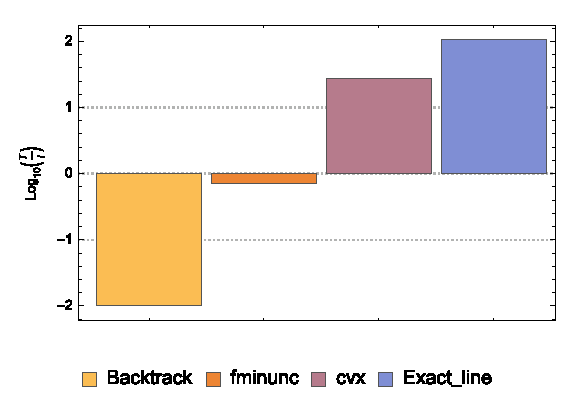
\includegraphics[width=8cm]{f1.eps}
\caption{\footnotesize{Normalized total computation time for each test. The total computation time was divided by the number of iterations. Since not all methods converged to the minimum this gives us the cost of each step and then they can be compared. A Backtrack iteration took as little as $10^{-2}s$ while a Exact line iteration took as much as $10^2s$ that is 4 orders of magnitude of difference. \label{f1}}}
\end{center}
\end{figure}

\subsection*{Final result}
The minimum was attained using \texttt{CVX}, (figure \ref{f2}) the solution of \texttt{fminunc} is just suboptimal by a factor of $10^1$. Both \texttt{Backtrack} and \texttt{Exact line} failed to converge and were stopped. The minimum difference of \texttt{Backtrack} after $2.5\times 10^4$ iterations is around $10^4$ whereas \texttt{Exact line} developed the worse carrying and error of $10^5$ after $200$ costly iterations.

\begin{figure}[!ht]
\begin{center}
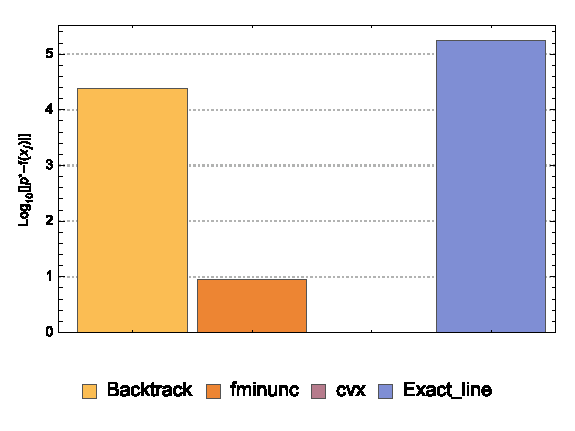
\includegraphics[width=8cm]{f2.eps}
\caption{\footnotesize{Final result. Since not all methods converged, here we plot the difference between the final result of the algorithm and the optimum $p^*$ }\label{f2}}
\end{center}
\end{figure}

\subsection*{First Test}
The first test found the solution $p^*=-226,894$ in just $1.3\times 10^2s$.

\subsection*{Second Test}
The second test found the solution $p^*=-226,885$ in $1.6\times 10^3s$. That is, suboptimal in 9 units. 

\subsection*{Third Test}

A plot of the convergence of the 16 essays is shown in figure \ref{f3}, distribution of final results in figure \ref{f4} and a plot of the comparison of final results and time cost for each essay in figure \ref{f5}.

\begin{figure}[!ht]
\begin{center}
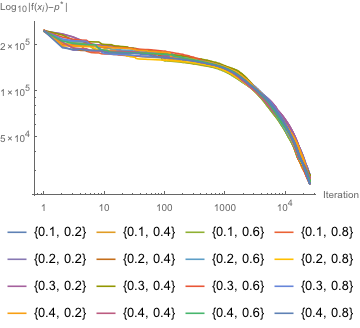
\includegraphics[width=8cm]{f3.png}
\caption{\footnotesize{Convergence plot for \texttt{Backtrack} algorithm. Several combinations of the parameters $\{\alpha_i,\beta_i\}$ were used. The function value though remains almost indistiguishable in the long run.}\label{f3}}
\end{center}
\end{figure}

\begin{figure}[!ht]
\begin{center}
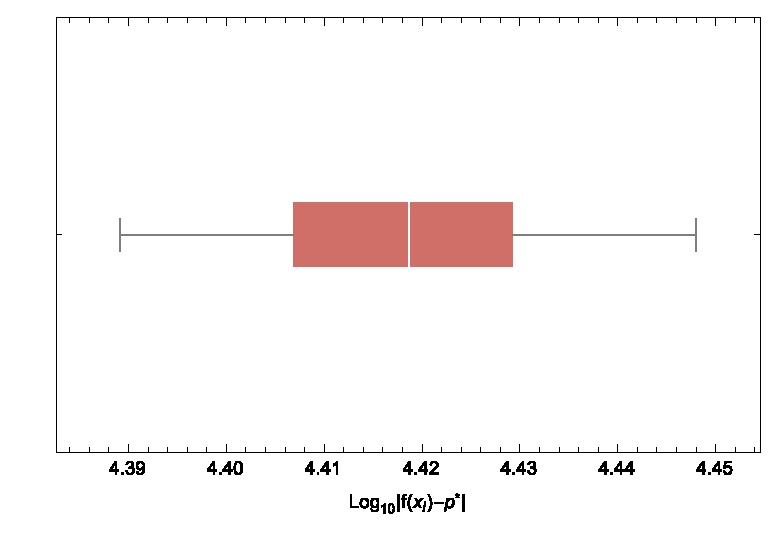
\includegraphics[width=8cm]{f4.eps}
\caption{\footnotesize{Distribution of the final result of the 16 parameter combinations of the Third Test. The logarithm of the difference with the optimal is plotted. As we can see, all final points are \emph{close}, at most $10^{3.55}$.}\label{f4}}
\end{center}
\end{figure}
\,
\begin{figure}[!ht]
\begin{center}
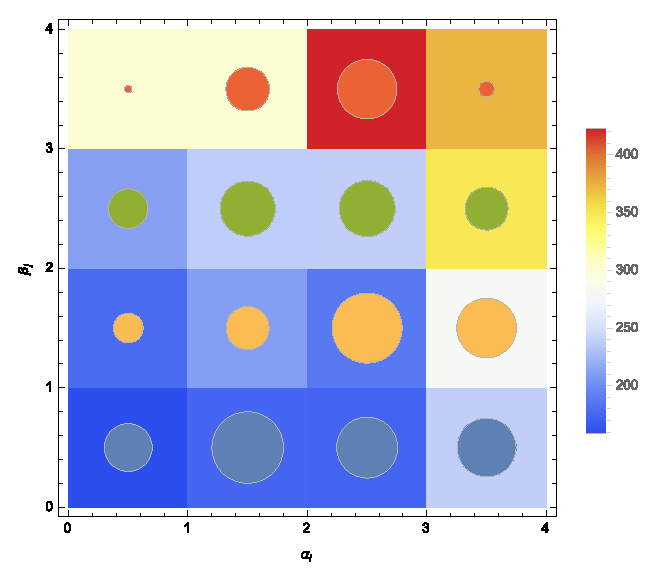
\includegraphics[width=8cm]{f5.eps}
\caption{\footnotesize{Combined Plot: Bubble plot of the normalized final result of each essay, and heat map of the time cost for each essay. We can see that the minimum final result is attained in the essay $\{\alpha_i,\beta_j\}=\{0.1,0.8\}$. The most costly essay is in $\{0.3,0.8\}$. The maximum final result is in $\{0.2,0.4\}$, The least costly essay is in $\{0.1,0.2\}$}\label{f5}}
\end{center}
\end{figure}

\subsection*{Fourth Test}
\texttt{Exact Line} search was the most costly and inexact. It took almost 6 hours to produce a result as good as any other algorithm. A comparison of the convergence of the three algorithms is plotted in figure \ref{f6}

\begin{figure}[!ht]
\begin{center}
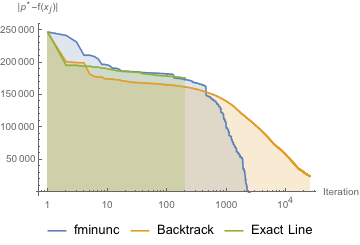
\includegraphics[width=9cm]{f6.png}
\caption{\footnotesize{Convergence comparison of the three methods. This is the most conclusive of all plots. \texttt{fminunc} converges fastly to global minimum, The best \texttt{Backtrack}} essay performs better in some region but after a change in regime, is passed by \texttt{fminunc}, fails to attain minimum in 25,000 iterations. \texttt{Exact Line} performs almost similar and between the previous two, but it's stopped 5.8 hours later after 200 iterations.\label{f6}}
\end{center}
\end{figure}

\section*{Conclusions}
\footnotesize{
\begin{enumerate}
\item For solving this problem it became essential to study the properties of the domain and the influence of the parameters prior to the implementation.
\item We implemented four different algorithms to solve a inequality constraint minimization problem and it's equivalent unconstrained minimization problem.
\item The association with the Inequality constraint minimization problem with the \emph{logarithmic barrier function} ensures the attainability of the minimum.
\item As noted by \cite{Boyd2002} exact line search develops awfully in practice, because the complexity of the problem grows rapidly.
\item As expected \texttt{CVX} is the only method to attain the minimum in reasonable time.
\item We can say the influence of the parameters $\alpha, \beta$ in \texttt{backtrack} method is not significant, specially in the long run.
\item Also, we can observe that all solutions of the different parameter setting in \texttt{backtrack} method remain close in the long run. 
\item Though, there exists variations in this solutions, not necessarily the most expensive computation carries the most accurate result. 
\item The solver of \texttt{fminunc} uses a \emph{quasi-newton} method, which results in at least a 10 times better than the best gradient descent method explored here.
\end{enumerate}
}
\bibliography{/Users/Poincare/Dropbox/Tex/library.bib}
\footnotesize{
\bibliographystyle{unsrt}
}



\end{document}